%%%%%%%%%%%%%%%%%%%%%%%%%%%%%%%%%%%%%%%%%
% Beamer Presentation
% LaTeX Template
% Version 1.0 (10/11/12)
%
% This template has been downloaded from:
% http://www.LaTeXTemplates.com
%
% License:
% CC BY-NC-SA 3.0 (http://creativecommons.org/licenses/by-nc-sa/3.0/)
%
%%%%%%%%%%%%%%%%%%%%%%%%%%%%%%%%%%%%%%%%%

%----------------------------------------------------------------------------------------
%	PACKAGES AND THEMES
%----------------------------------------------------------------------------------------

\documentclass{beamer}

\mode<presentation> {
	
	% The Beamer class comes with a number of default slide themes
	% which change the colors and layouts of slides. Below this is a list
	% of all the themes, uncomment each in turn to see what they look like.
	
	%\usetheme{default}
	%\usetheme{AnnArbor}
	%\usetheme{Antibes}
	%\usetheme{Bergen}
	%\usetheme{Berkeley}
	%\usetheme{Berlin}
	%\usetheme{Boadilla}
	%\usetheme{CambridgeUS}
	%\usetheme{Copenhagen}
	%\usetheme{Darmstadt}
	%\usetheme{Dresden}
	%\usetheme{Frankfurt}
	%\usetheme{Goettingen}
	%\usetheme{Hannover}
	%\usetheme{Ilmenau}
	%\usetheme{JuanLesPins}
	%\usetheme{Luebeck}
	\usetheme{Madrid}
	%\usetheme{Malmoe}
	%\usetheme{Marburg}
	%\usetheme{Montpellier}
	%\usetheme{PaloAlto}
	%\usetheme{Pittsburgh}
	%\usetheme{Rochester}
	%\usetheme{Singapore}
	%\usetheme{Szeged}
	%\usetheme{Warsaw}
	
	% As well as themes, the Beamer class has a number of color themes
	% for any slide theme. Uncomment each of these in turn to see how it
	% changes the colors of your current slide theme.
	
	%\usecolortheme{albatross}
	\usecolortheme{beaver}
	%\usecolortheme{beetle}
	%\usecolortheme{crane}
	%\usecolortheme{dolphin}
	%\usecolortheme{dove}
	%\usecolortheme{fly}
	%\usecolortheme{lily}
	%\usecolortheme{orchid}
	%\usecolortheme{rose}
	%\usecolortheme{seagull}
	%\usecolortheme{seahorse}
	%\usecolortheme{whale}
	%\usecolortheme{wolverine}
	
	%\setbeamertemplate{footline} % To remove the footer line in all slides uncomment this line
	%\setbeamertemplate{footline}[page number] % To replace the footer line in all slides with a simple slide count uncomment this line
	
	%\setbeamertemplate{navigation symbols}{} % To remove the navigation symbols from the bottom of all slides uncomment this line
}

\usepackage{graphicx} % Allows including images
\usepackage{subfigure}
\usepackage{booktabs} % Allows the use of \toprule, \midrule and \bottomrule in tables
\usepackage{bm}

%----------------------------------------------------------------------------------------
%	TITLE PAGE
%----------------------------------------------------------------------------------------

\title[PGD]{Non-Convex Projected Gradient Descent for Generalized Low-Rank Tensor Regression} 

\author{Ganchao Wei} 
\date{December 1, 2021}

\begin{document}
	
	\begin{frame}
		\titlepage % Print the title page as the first slide
	\end{frame}
	
	\begin{frame}
		\frametitle{Overview} % Table of contents slide, comment this block out to remove it
		\tableofcontents
	\end{frame}
	
	%--------------------------------------------------------------------
	%	PRESENTATION SLIDES
	%--------------------------------------------------------------------
	
	\section{Tensor regression}
	
	\begin{frame}
		\frametitle{Generalized Tensor Regression}
		For a scalar response $Y$, given a covariate tensor $X\in\mathbb{R}^{d_1\times d_2\times \ldots \times d_N}$, the generalized tensor regression is:
		$$p(Y|X,T)=h(Y)\exp\{Y<X,T> - a(<X,T>)\}$$
		, where $a(\cdots)$ is a strictly convex and differentiable log-partition function, $h(\cdot)$ is a nuisance parameter, and $T\in\mathbb{R}^{d_1\times d_2\times \ldots \times d_N}$ is the parameter tensor of interest. Hence The negative log-likelihood risk object is:
		$$L(A) = \frac{1}{n}\sum_{i=1}^{n}[a(<X^{(i)}, A>) - Y^{(i)}<X^{(i)}, A> - \log h(Y^{(i)})]$$
		Some notations:
		\begin{itemize}
			\item 
			$<\cdot,\cdot>$: inner product
			\item
			$||A||_F = <A,A>^{1/2}$
			\item
			$||A||_n^2$:empirical norm
			\item
			$A_{A}$: projection of a tensor A onto A.
		\end{itemize}
	\end{frame}
	
	\begin{frame}
		\frametitle{Tensor Algebra}
		There are 2 standard tensor decompositions (e.g. third-order tensors):
		\begin{itemize}
			\item
			canonical polyadic (CP) decomposition:
			\begin{figure}
				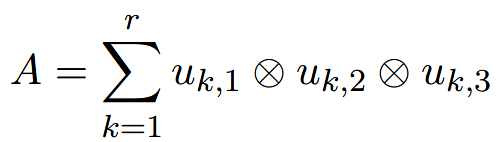
\includegraphics[width=.4\linewidth]{image001.png}
			\end{figure}
			\item
			Tucker decomposition:
			\begin{figure}
				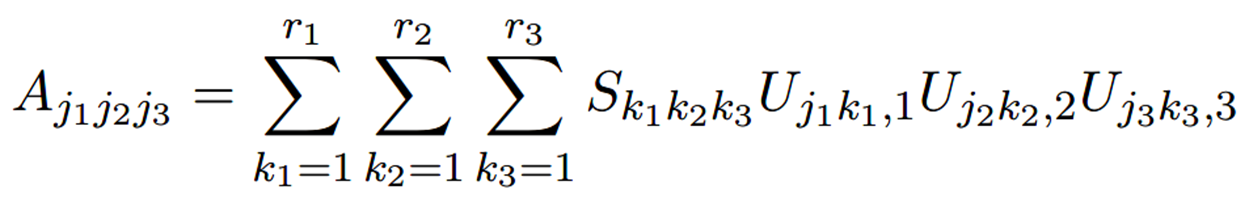
\includegraphics[width=.7\linewidth]{image002.png}
			\end{figure}
		\end{itemize}
		Moreover, there are some tensor operators:
		\begin{itemize}
			\item
			matricization: $M_m(A)$
			\item
			vectorization: $vec(A)$
			\item
			slices:
			 \begin{figure}
			 	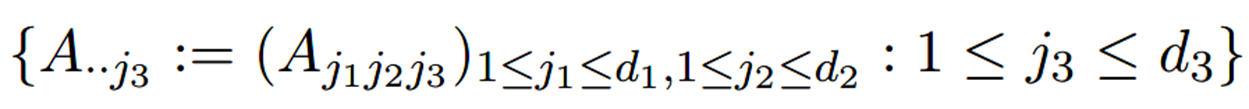
\includegraphics[width=.7\linewidth]{image003.png}
			 \end{figure}
		\end{itemize}
	\end{frame}
	
	
	\begin{frame}
		\frametitle{Low-dimensional Structural Assumption}
		Consider 3 (non-convex) specific examples of low-rank structure:
		\begin{itemize}
			\item 
			Low-rank structure on the matrix slices:
			 \begin{figure}
				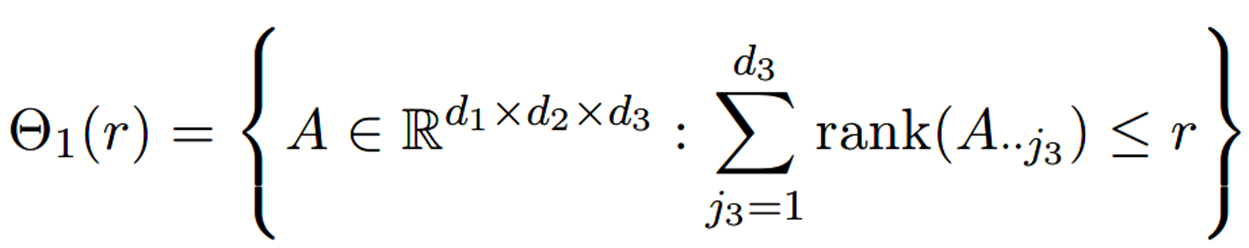
\includegraphics[width=.6\linewidth]{image004.png}
			\end{figure}
			\item
			Bound the maximum of the rank of each slice and sparsity along the matrix slices:
			 \begin{figure}
				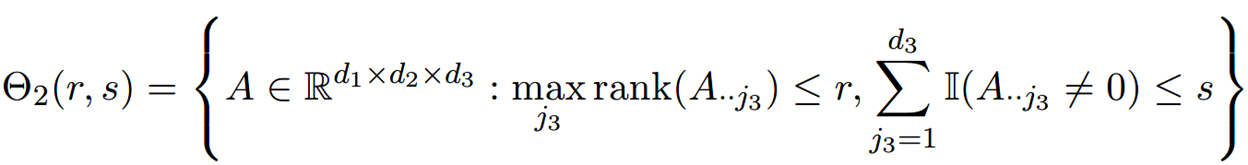
\includegraphics[width=.8\linewidth]{image005.png}
			\end{figure}
			\item
			Tucker ranks are upper bounded:
			 \begin{figure}
				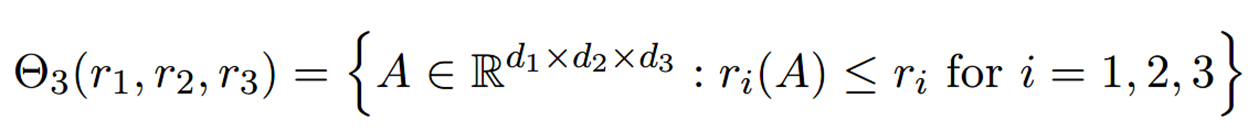
\includegraphics[width=.7\linewidth]{image006.png}
			\end{figure}
		\end{itemize}
	\end{frame}
	
	
	\begin{frame}
		\frametitle{Projected Gradient Descent}
		Minimize a general loss function $f(A)$ subject to constraint $A\in \Theta$:
		\begin{figure}
			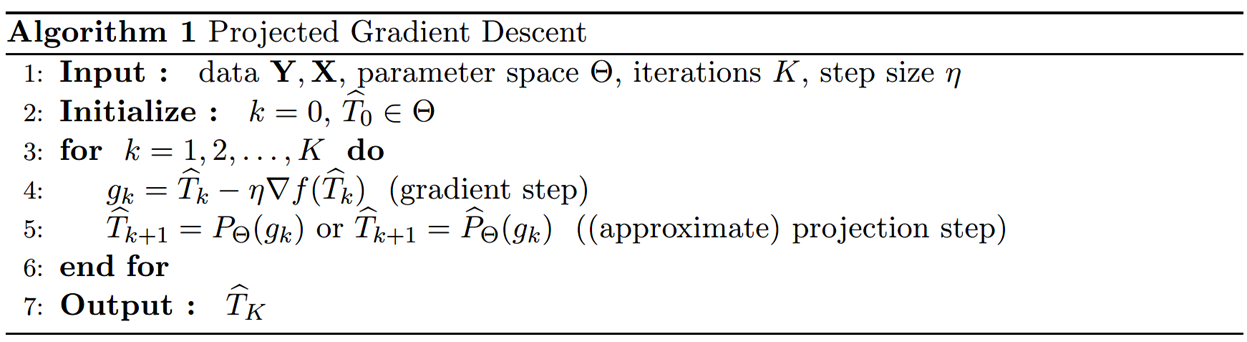
\includegraphics[width=.9\linewidth]{image007.png}
		\end{figure}
		Denote 2 specific projections as:
		\begin{itemize}
			\item 
			projection to the set of s-sparse vectors:
			\begin{figure}
				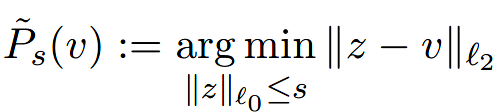
\includegraphics[width=.4\linewidth]{image008.png}
			\end{figure}
			\item
			rank-r projection of a matrix:
			\begin{figure}
				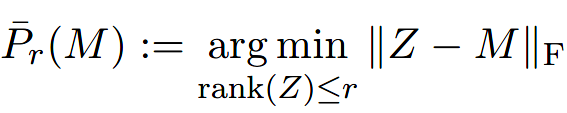
\includegraphics[width=.4\linewidth]{image009.png}
			\end{figure}
		\end{itemize}
	\end{frame}
	
	\begin{frame}
		\frametitle{Properties for $\Theta$ and its projection}
		View $\Theta$ as a member of a collection of subspaces $\{\Theta(t): t\in \Xi\}$. Then the 3 low-dimensional structures:
		\begin{itemize}
			\item 
			$\Theta_1(r):$
			\begin{figure}
				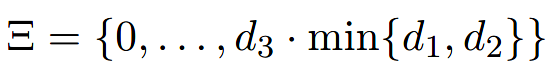
\includegraphics[width=.35\linewidth]{image010.png}
			\end{figure}
			\item
			$\Theta_2(r, s):$
			\begin{figure}
				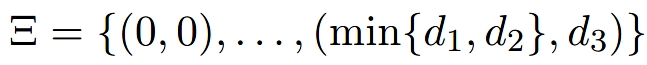
\includegraphics[width=.4\linewidth]{image011.png}
			\end{figure}
			\item
			$\Theta_3(r_1, r_2, r_3):$
			\begin{figure}
				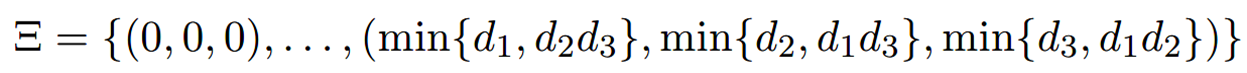
\includegraphics[width=.8\linewidth]{image012.png}
			\end{figure}
		\end{itemize}
	\end{frame}
	
	
	\begin{frame}
		\frametitle{Properties for $\Theta$ and its projection}
		Further, there are some definitions:
		\begin{figure}
			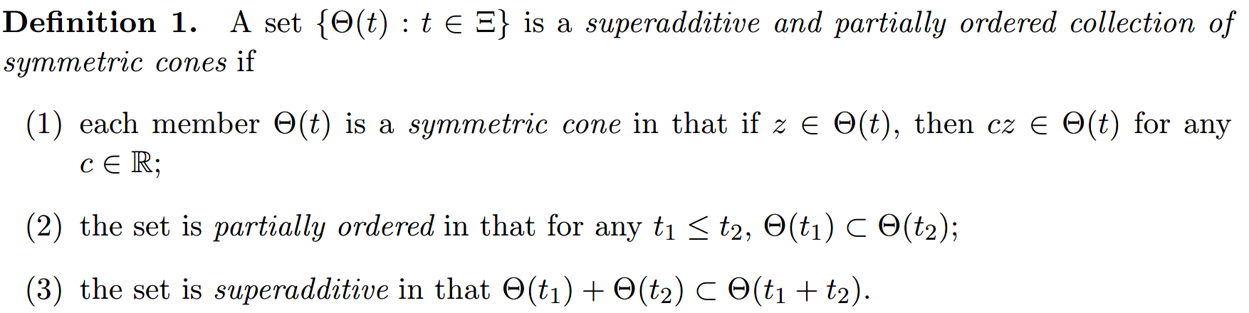
\includegraphics[width=.9\linewidth]{image013.png}
		\end{figure}
		And the definition of contractive projection:
		\begin{figure}
			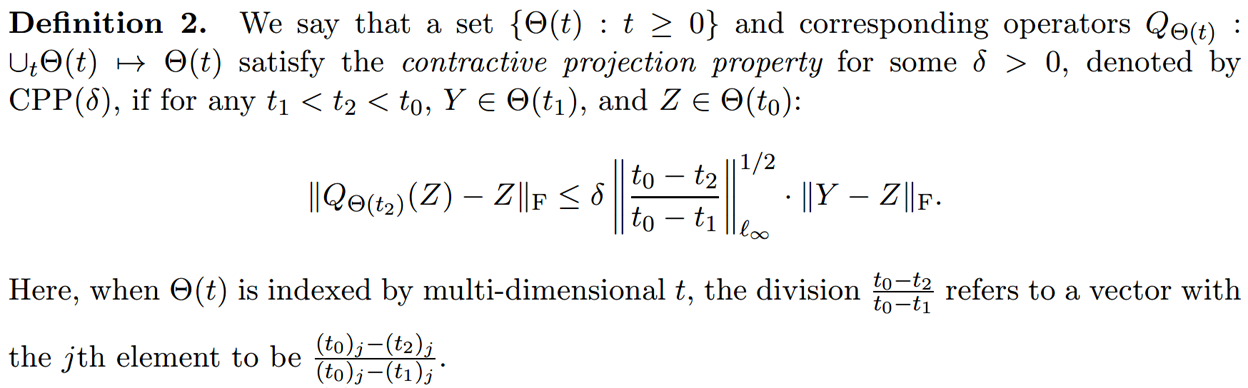
\includegraphics[width=.9\linewidth]{image014.png}
		\end{figure}
	\end{frame}
	
	\begin{frame}
		\frametitle{Restricted strong convexity}
		To guarantee the PGD performance, we further need  the restricted strong convexity and smoothness conditions (RSCS):
		\begin{figure}
			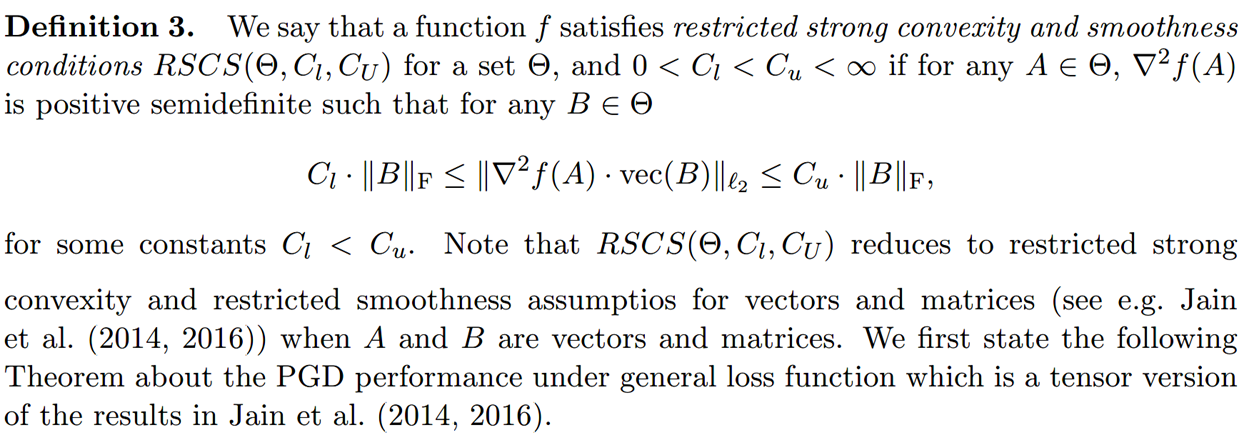
\includegraphics[width=1\linewidth]{image015.png}
		\end{figure}
	\end{frame}
	
	\begin{frame}
		\frametitle{Restricted strong convexity}
		Under this condition, we can give the error bound for general loss function:
		\begin{figure}
			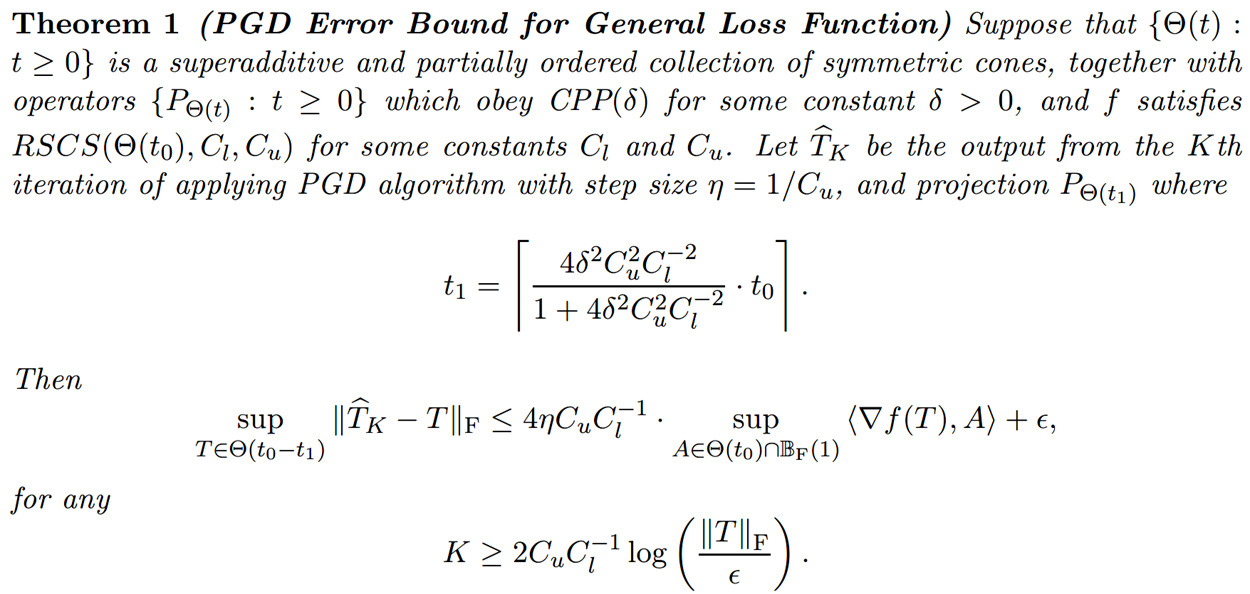
\includegraphics[width=1\linewidth]{image016.png}
		\end{figure}
		We then specialize $f$ to the generalized linear model.
	\end{frame}
	
	\begin{frame}
		\frametitle{Generalized linear models}
		For convenience, we assume \& define:
		\begin{itemize}
			\item 
			Gaussian design og independent samples tensors:
			\begin{figure}
				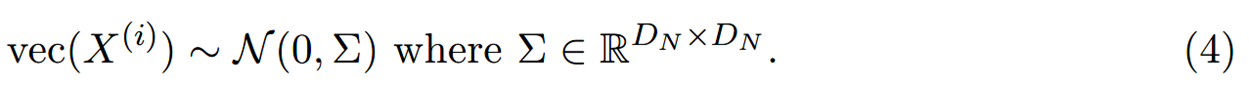
\includegraphics[width=.8\linewidth]{image017.png}
			\end{figure}
			\item
			$\Sigma$ has bounded eigenvalues:
			\begin{figure}
				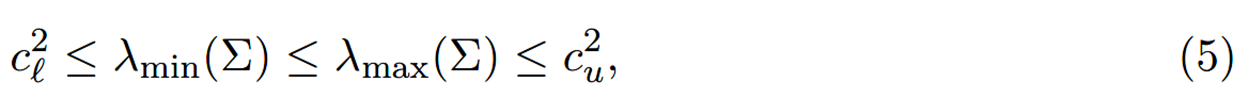
\includegraphics[width=.8\linewidth]{image018.png}
			\end{figure}
			\item
			Gaussian width:
			\begin{figure}
				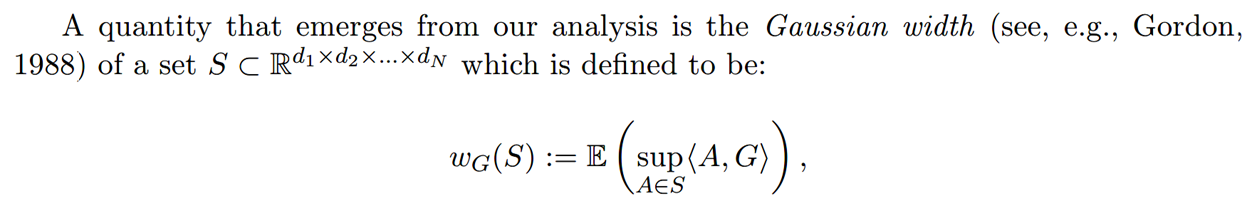
\includegraphics[width=1\linewidth]{image019.png}
			\end{figure}
		\end{itemize}
	\end{frame}
	
	\begin{frame}
		\frametitle{Generalized linear models}
		\begin{figure}
			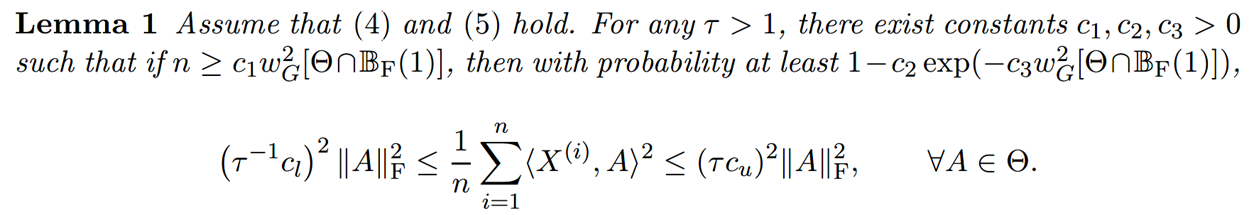
\includegraphics[width=.75\linewidth]{image020.png}
			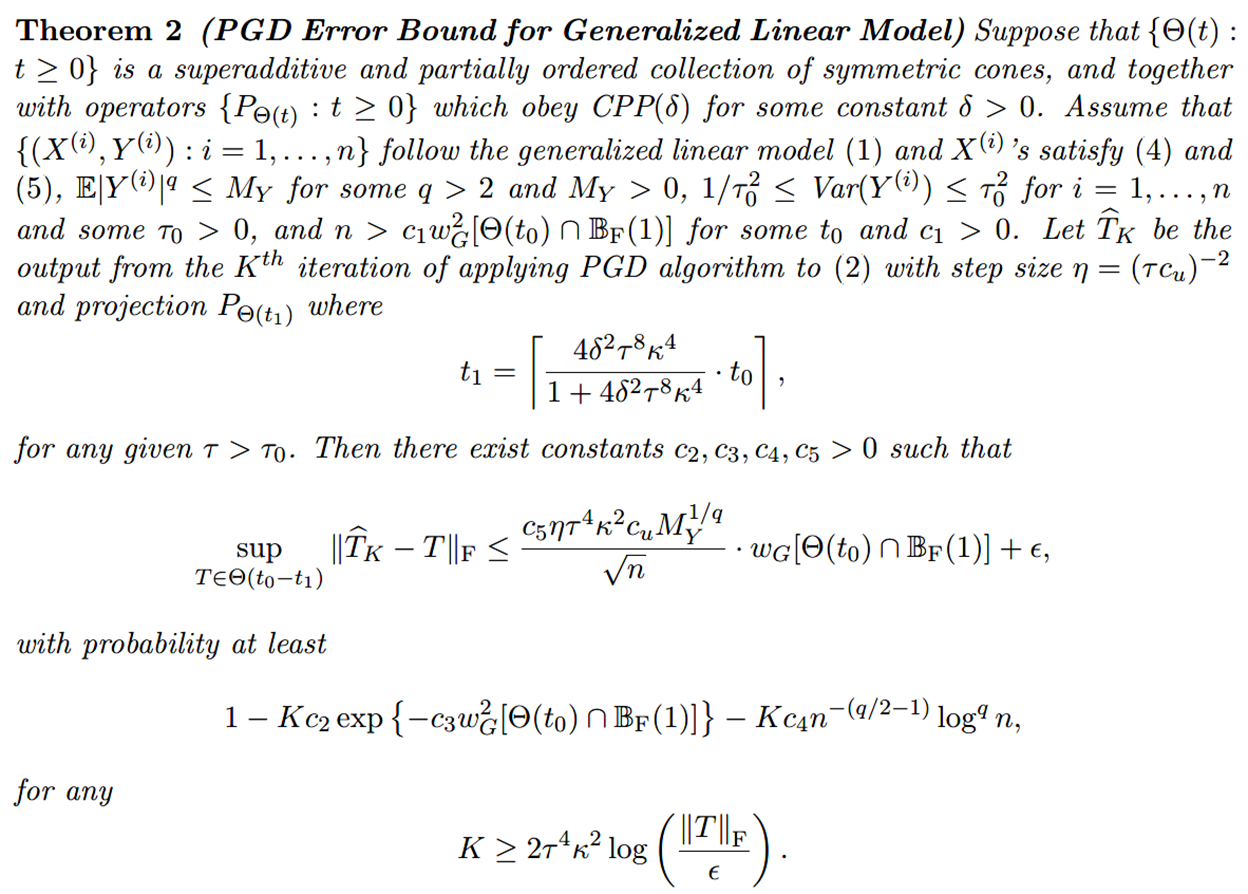
\includegraphics[width=.75\linewidth]{image021.png}
		\end{figure}
	\end{frame}
	
	\begin{frame}
		\frametitle{Normal linear regression}
		The moment conditions ensure the restricted strong convexity \& restricted smoothness conditions. When considering normal linear regression, these conditions could be further removed.
		\begin{figure}
			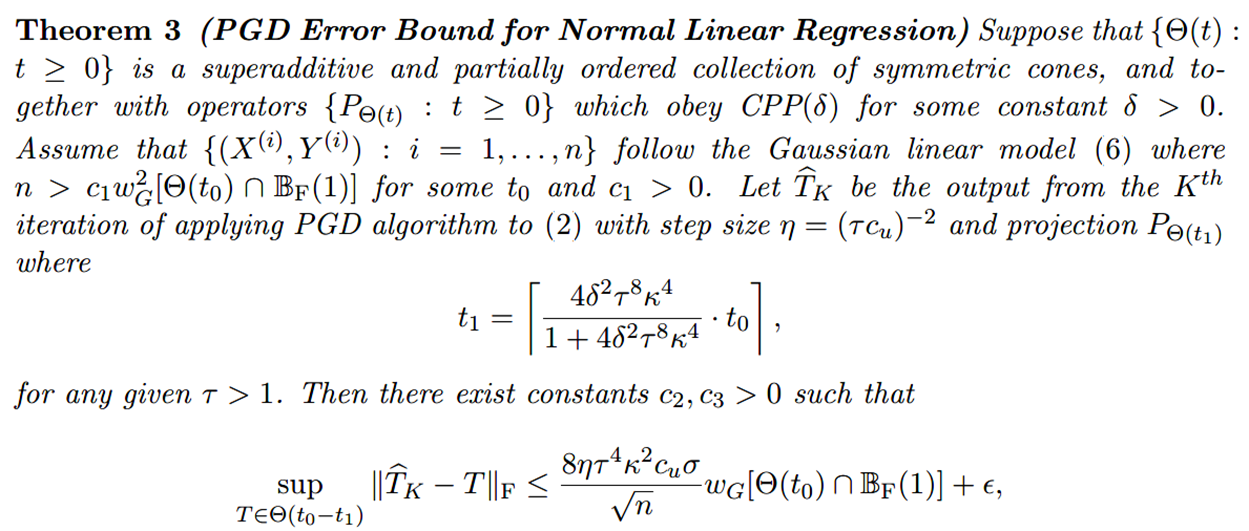
\includegraphics[width=.75\linewidth]{image022.png}
			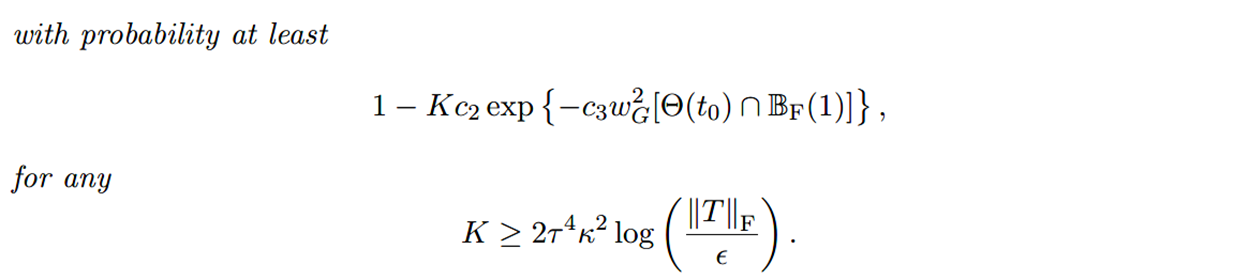
\includegraphics[width=.75\linewidth]{image023.png}
		\end{figure}
	\end{frame}
	
	\begin{frame}
		\frametitle{Normal linear regression}
		The convex regularization approach:
		\begin{figure}
			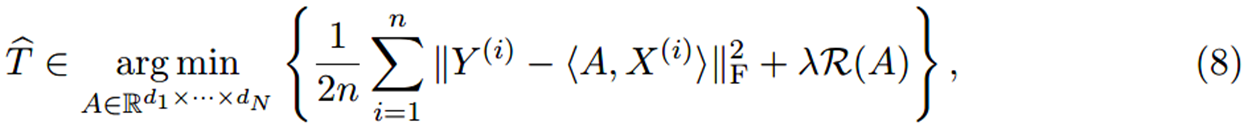
\includegraphics[width=.8\linewidth]{image024.png}
		\end{figure}
		The error bound:
		\begin{figure}
			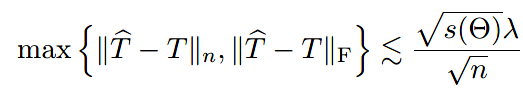
\includegraphics[width=.5\linewidth]{image025.png}
		\end{figure}
		when $\lambda=2\omega_G(\mathbb{B}_R(1))$
		\begin{figure}
			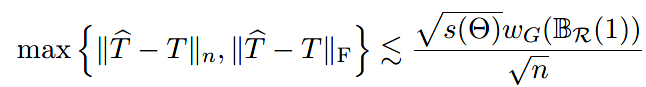
\includegraphics[width=.6\linewidth]{image026.png}
		\end{figure}
	\end{frame}
	
	\begin{frame}
		\frametitle{Normal linear regression}
		By
		\begin{figure}
			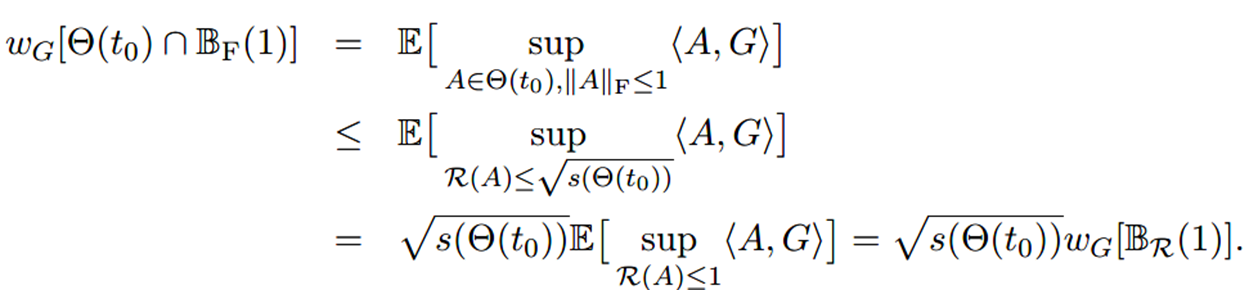
\includegraphics[width=.9\linewidth]{image027.png}
		\end{figure}
		The non-convex error bound is always no larger than the convex error bound.
	\end{frame}
	
	\begin{frame}
		\frametitle{Specific low rank structure}
		$\Theta_1(r)$ is identical to the case of low rank matrix estimation. For $\Theta_2(r,s)$:
		\begin{figure}
			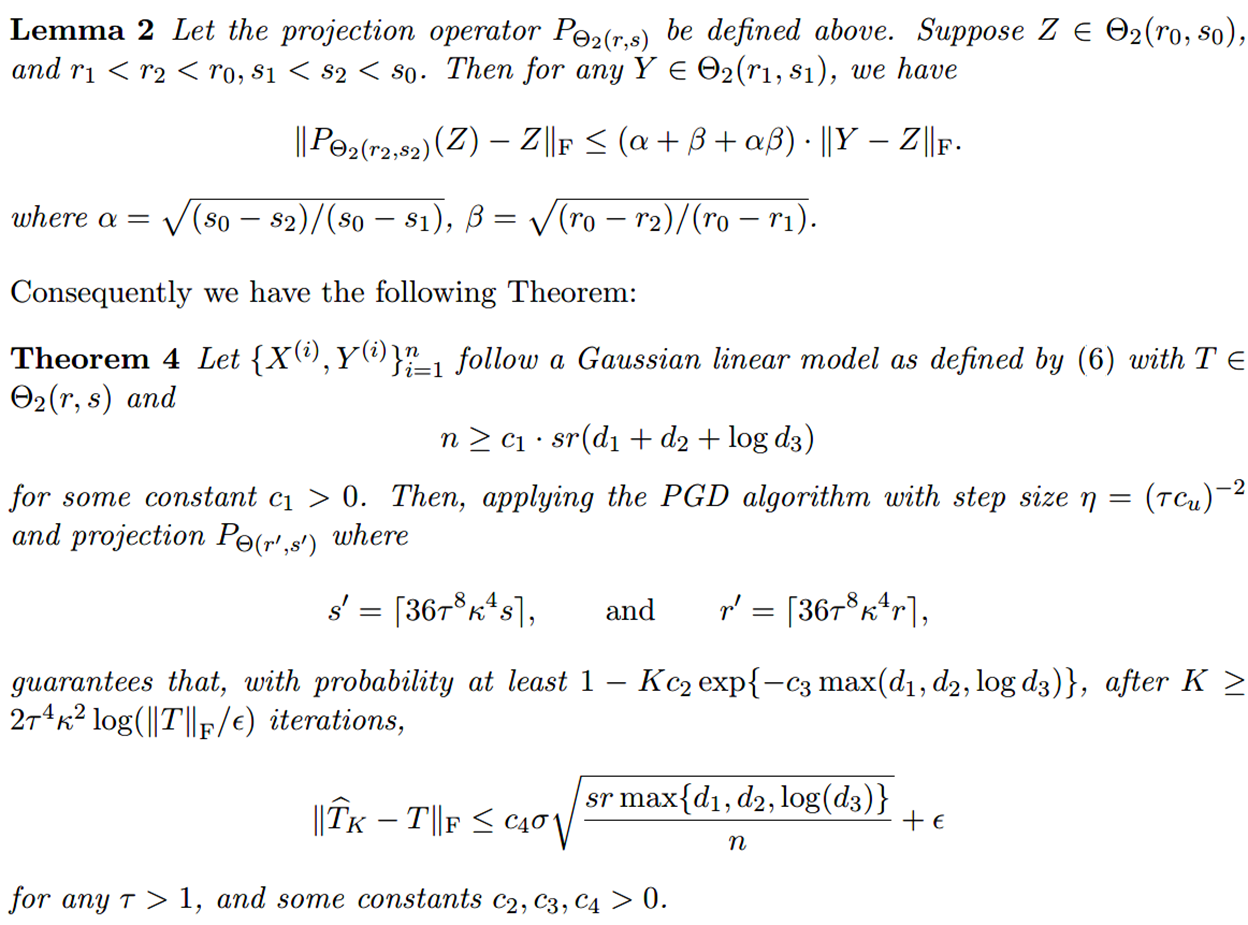
\includegraphics[width=.7\linewidth]{image028.png}
		\end{figure}
	
	\end{frame}
	
	\begin{frame}
		\frametitle{Specific low rank structure}
		The $\Theta_2(r,s)$ is not suitable for convex regularization, so only compare for $\Theta_1(r)$.
		\begin{figure}
			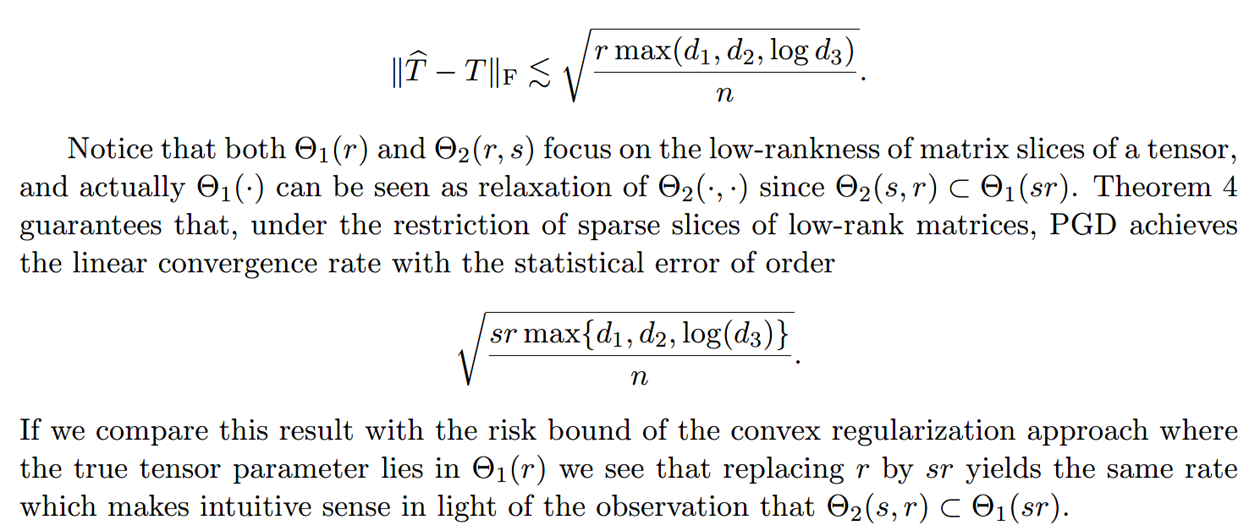
\includegraphics[width=1\linewidth]{image029.png}
		\end{figure}
	\end{frame}
	
	\begin{frame}
		\frametitle{Specific low rank structure}
		We further consider the low Tucker rank $\Theta_3(r_1, r_2, r_3)$:
		\begin{figure}
			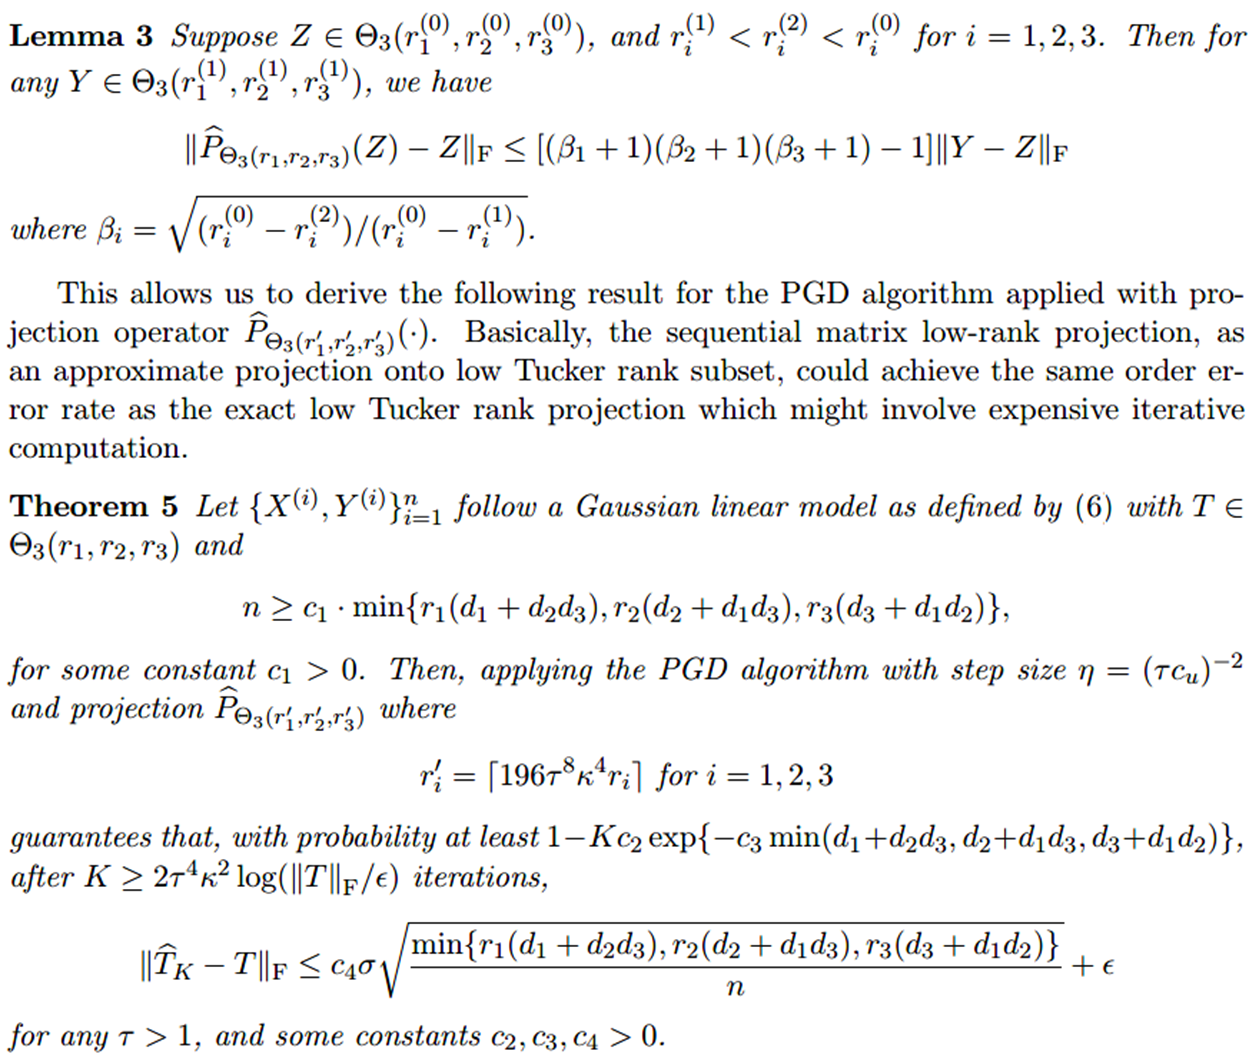
\includegraphics[width=.7\linewidth]{image030.png}
		\end{figure}
	\end{frame}
	
	
	\begin{frame}
		\frametitle{Specific low rank structure}
		The error bound for convex regularization:
		\begin{figure}
			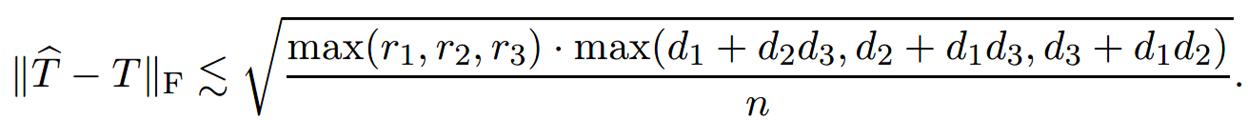
\includegraphics[width=.7\linewidth]{image031.png}
		\end{figure}
		Notice that min is replaced by max, so PGD is better.
	\end{frame}
	
	
	\begin{frame}
		\frametitle{Simulations}
		How to select step-size for PGD?
		\begin{itemize}
			\item 
			if $\eta$ is too large: divergence
			\item
			if $\eta$ is too small: slow convergence
		\end{itemize}
		2 directions:
		\begin{itemize}
			\item 
			start with large, decrease when divergence is observed
			\item
			start with small, increase but step back when divergence is observed.
		\end{itemize}
		
		For all simulations, generally we can see:
		\begin{itemize}
			\item 
			larger $\eta$ $\Rightarrow$ faster convergence
			\item
			larger $r'$ or $s'$ $\Rightarrow$ faster convergence: wrong rank/sparsity will do harm to the performance of PGD.
		\end{itemize}
	\end{frame}
	
	\begin{frame}
		\frametitle{Simulations}
		\begin{figure}
			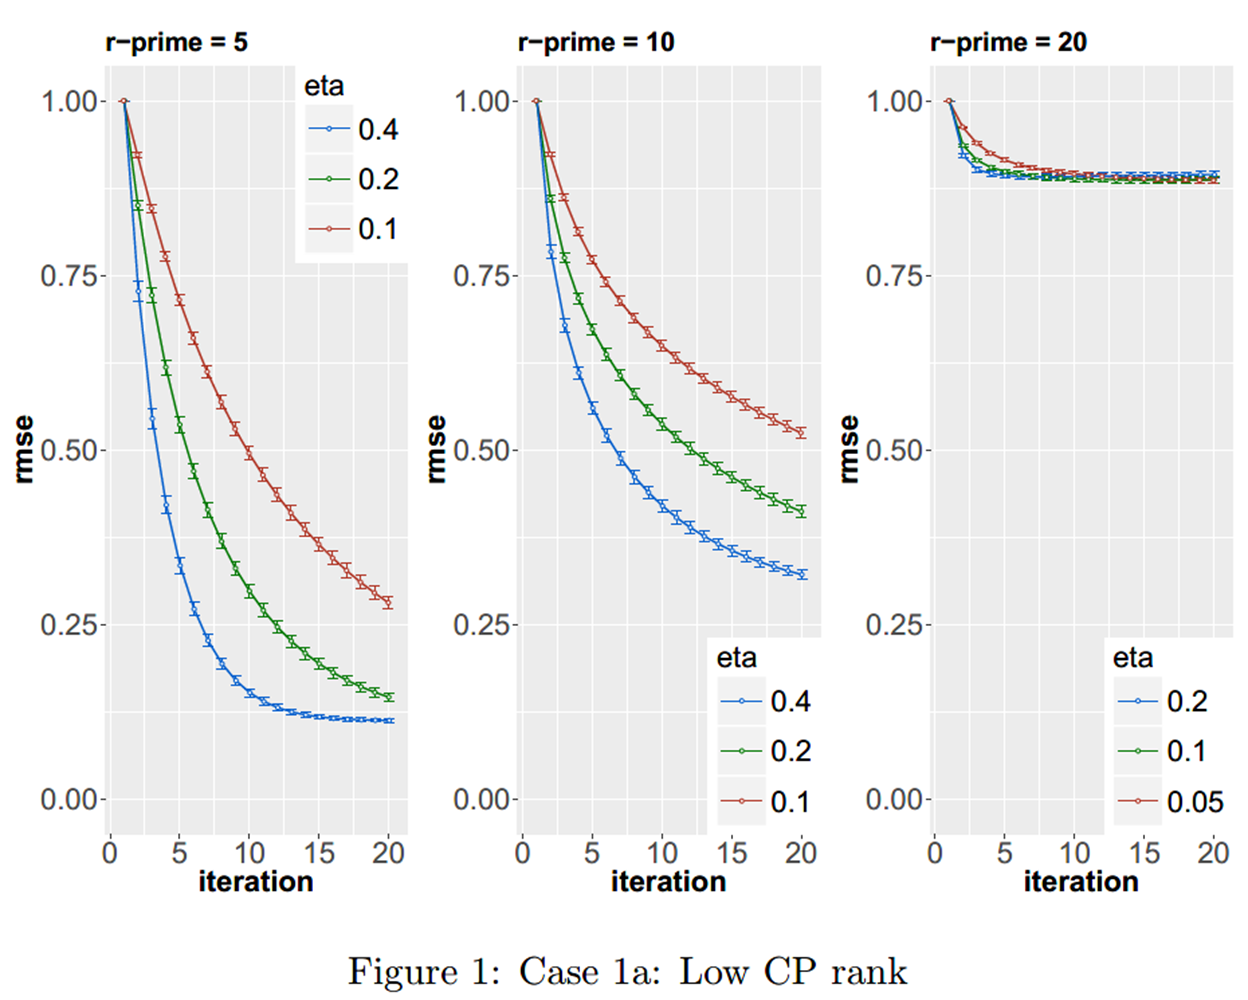
\includegraphics[width=.45\linewidth]{image032.png}
			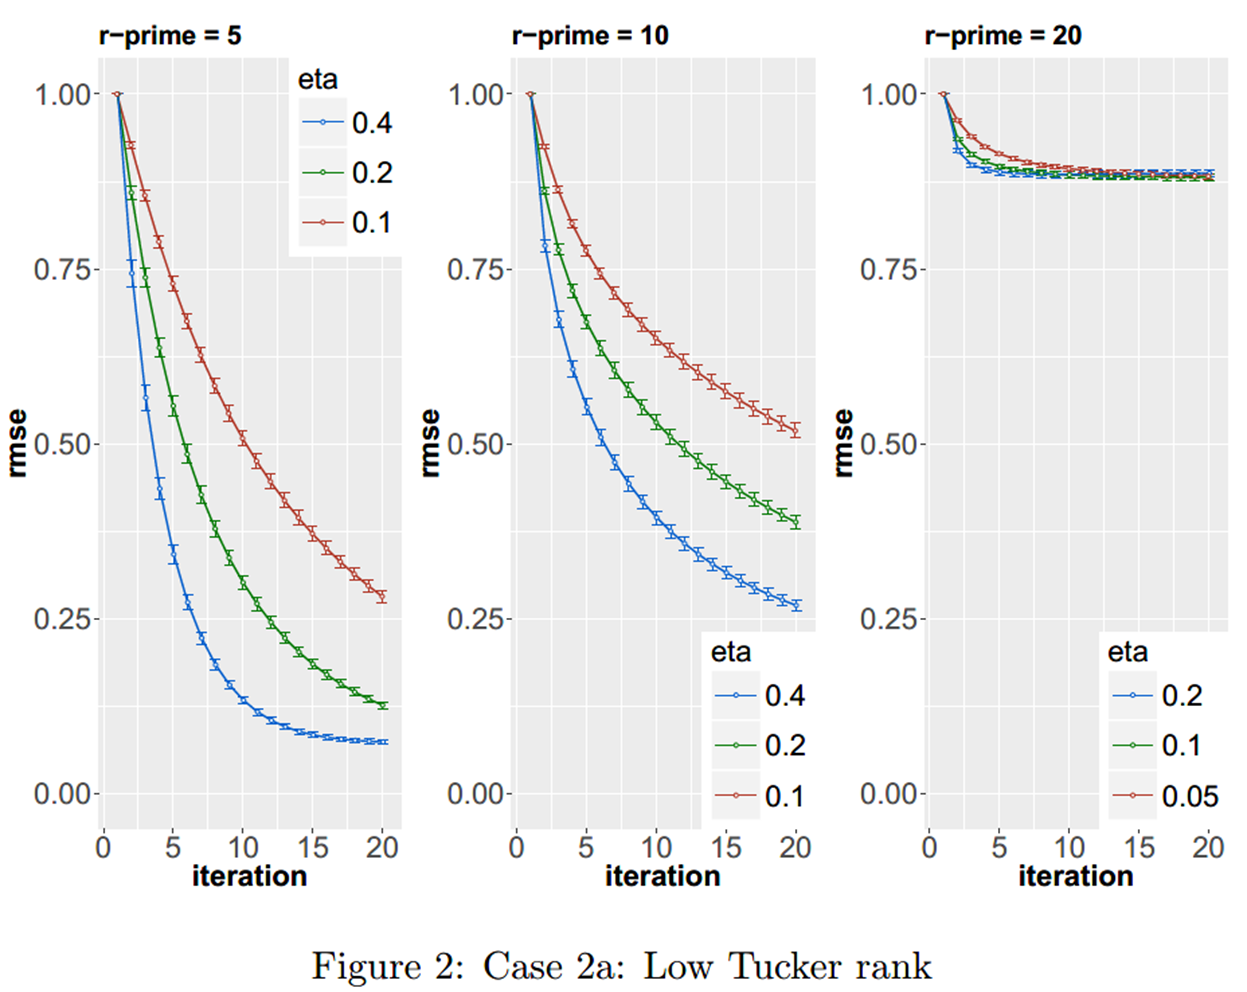
\includegraphics[width=.45\linewidth]{image033.png}
		\end{figure}
	\end{frame}
	
	\begin{frame}
		\frametitle{Simulations}
		\begin{figure}
			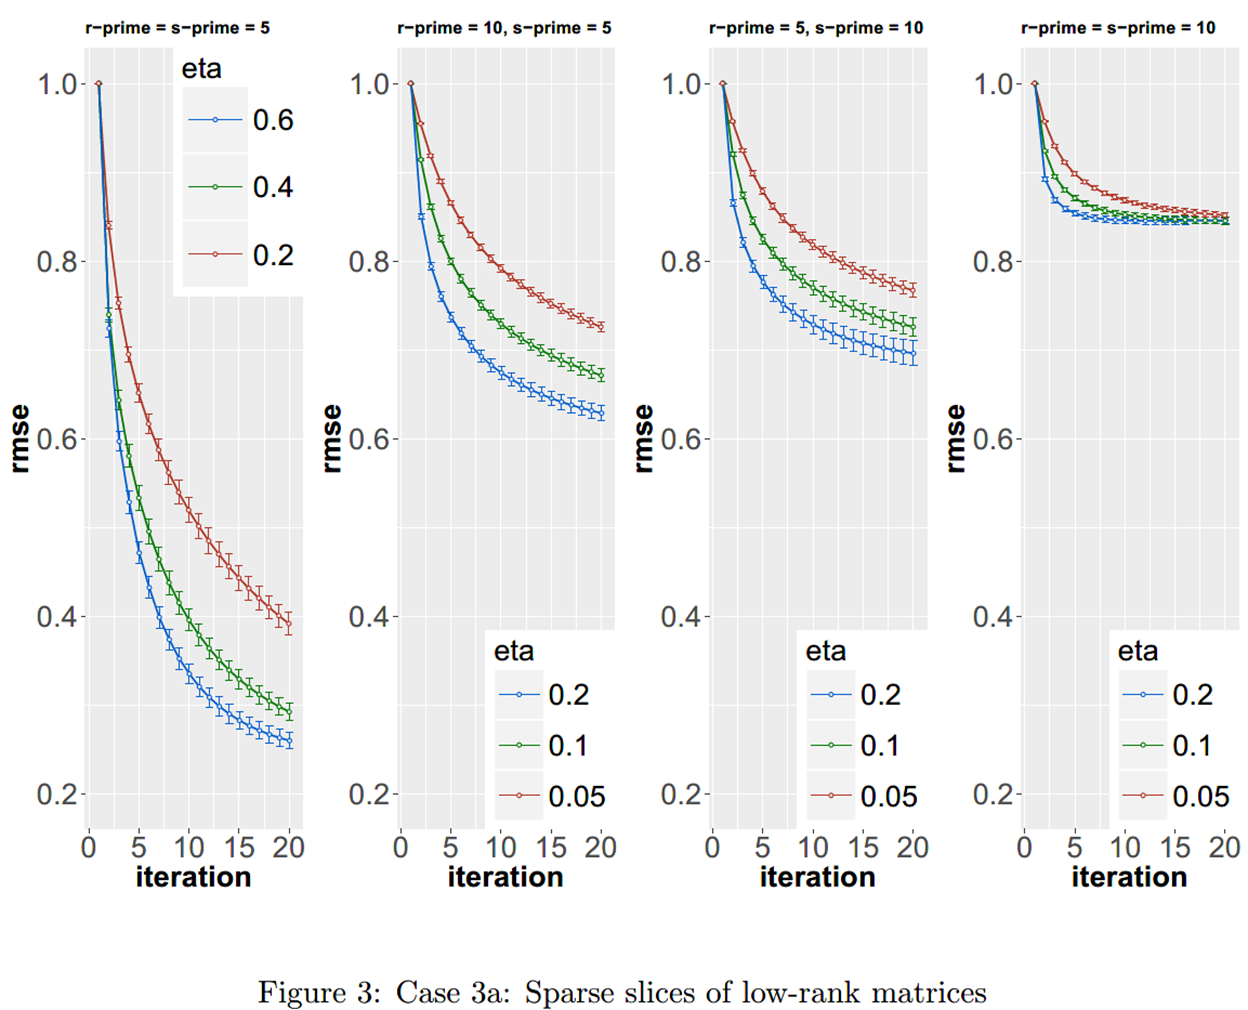
\includegraphics[width=.45\linewidth]{image034.png}
			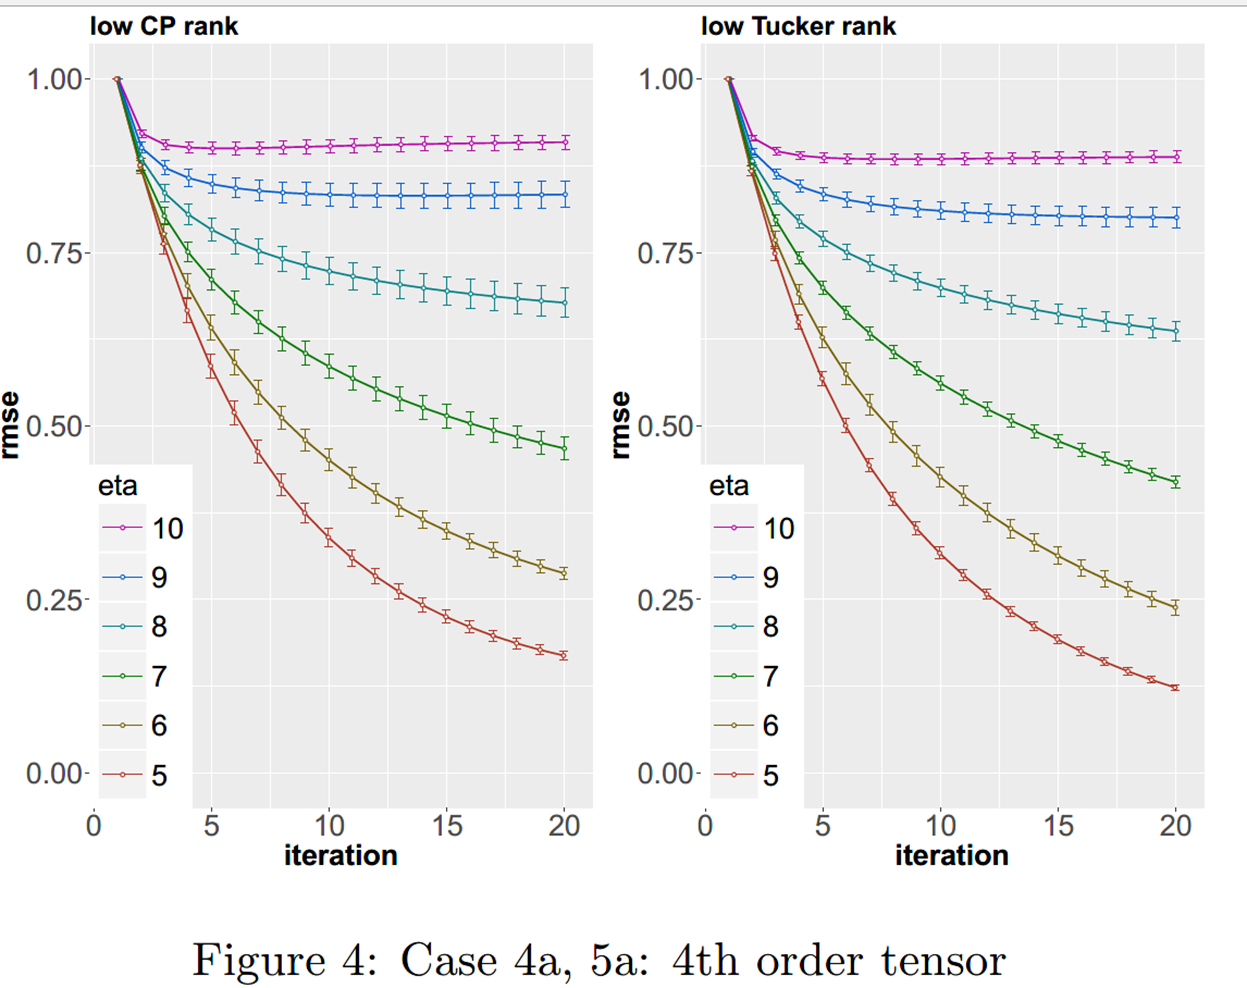
\includegraphics[width=.45\linewidth]{image035.png}
		\end{figure}
	\end{frame}
	
	
	\begin{frame}
		\frametitle{Simulations}
		\begin{figure}
			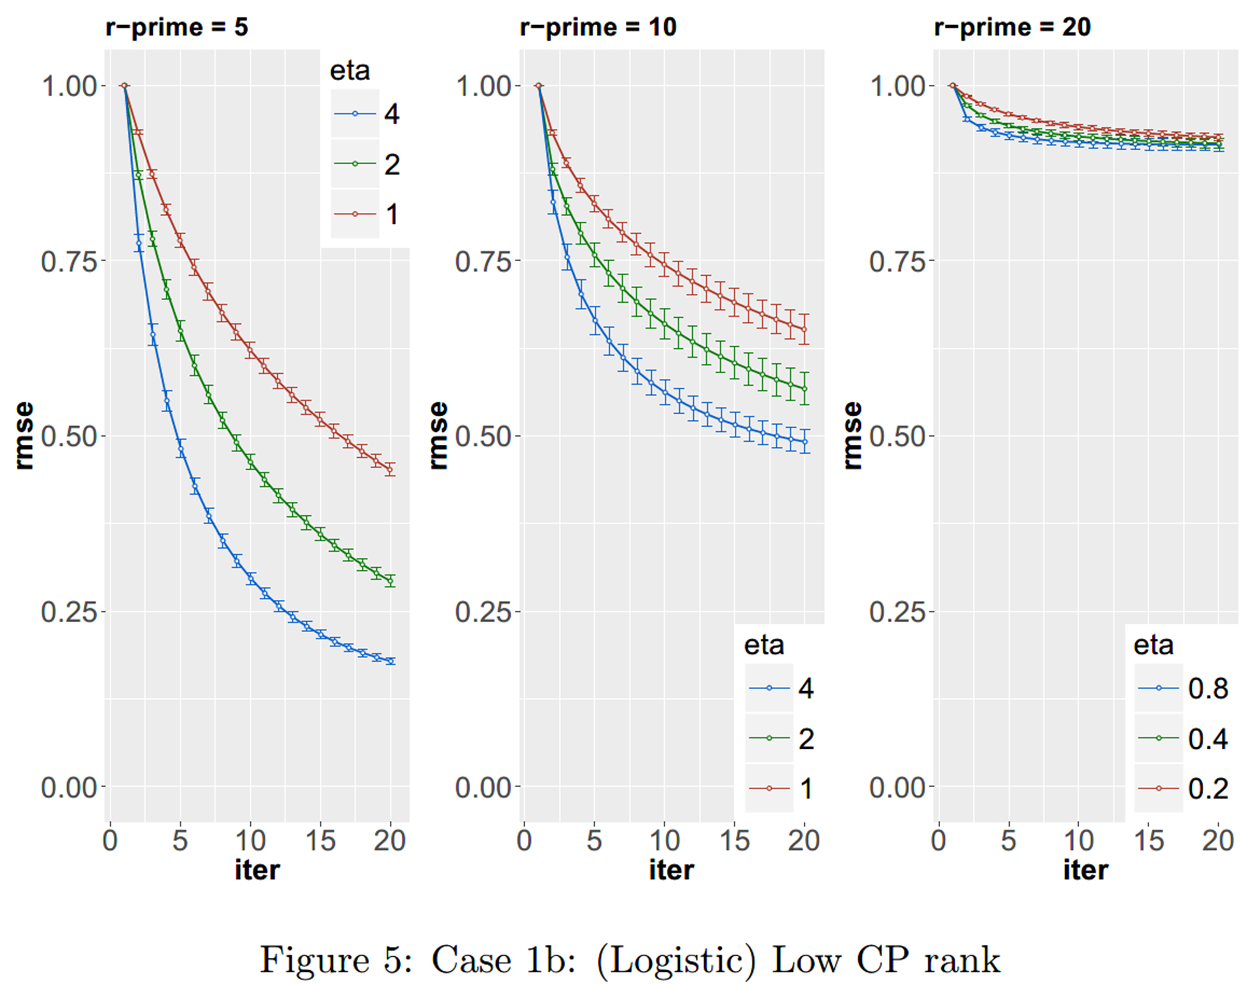
\includegraphics[width=.45\linewidth]{image036.png}
			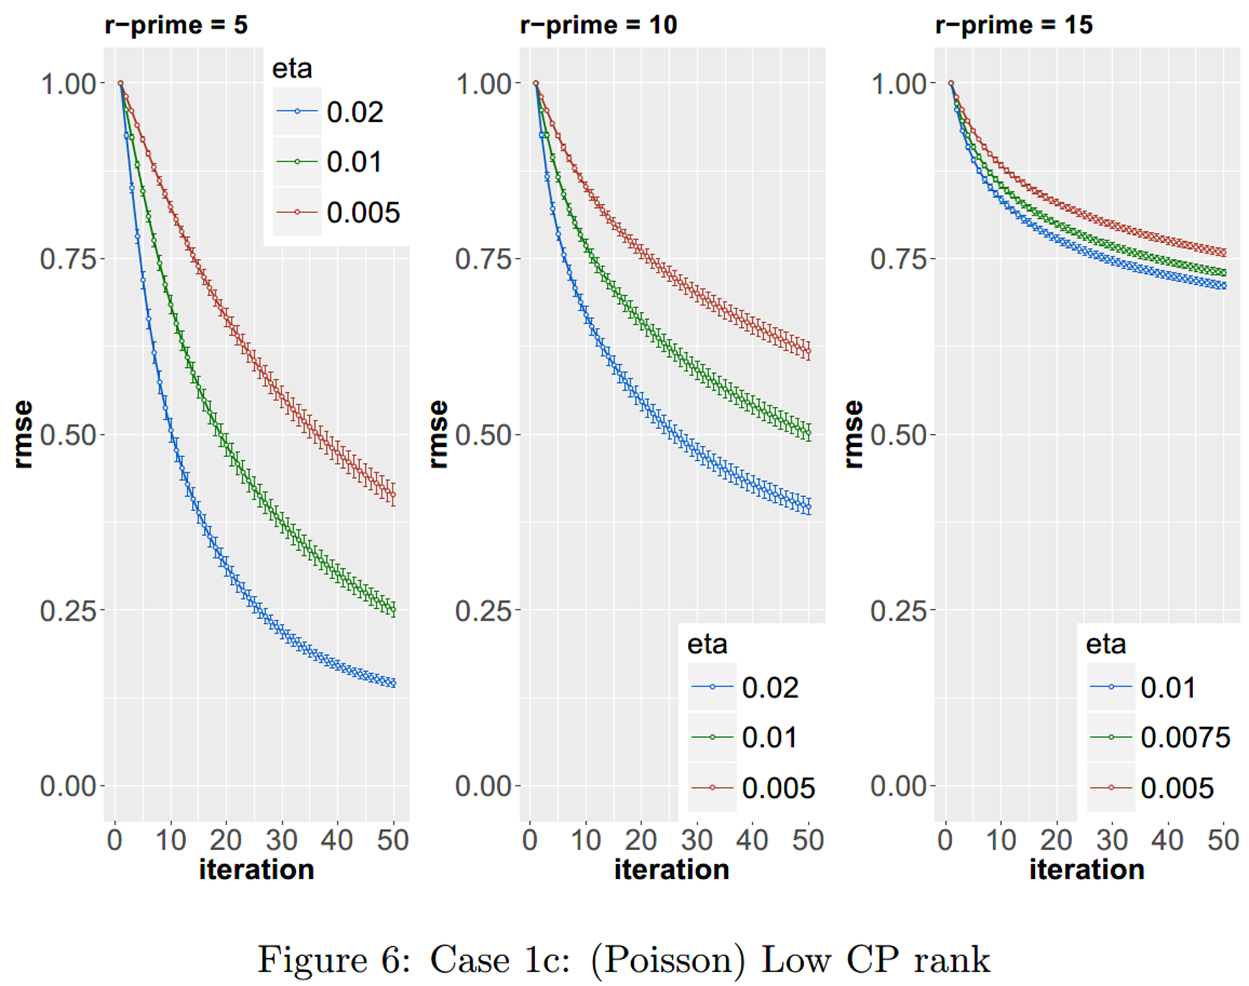
\includegraphics[width=.45\linewidth]{image037.png}
		\end{figure}
	\end{frame}
	
	\begin{frame}
		\frametitle{Simulations}
		\begin{figure}
			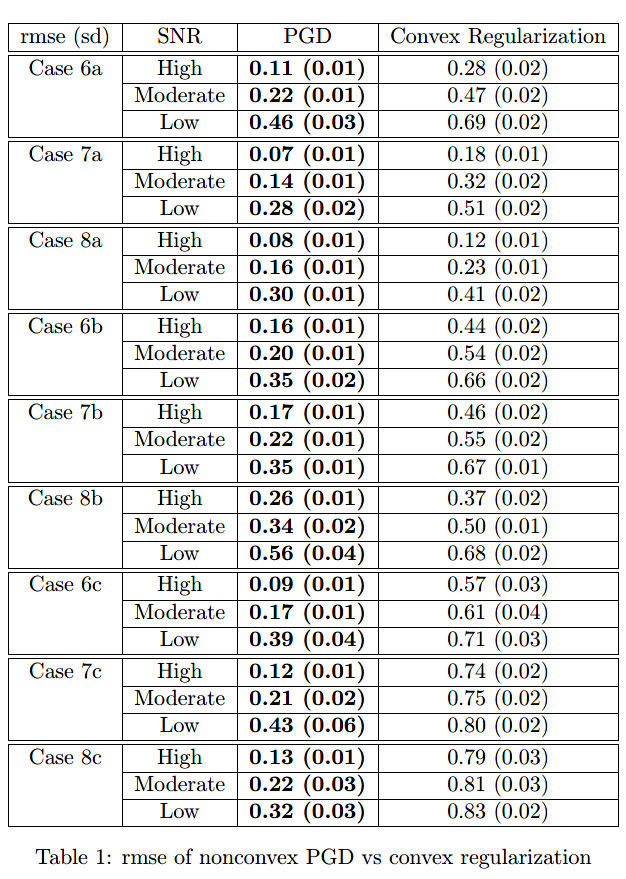
\includegraphics[width=.45\linewidth]{image038.png}
		\end{figure}
	\end{frame}
	
	\begin{frame}
		\frametitle{Simulations}
		\begin{figure}
			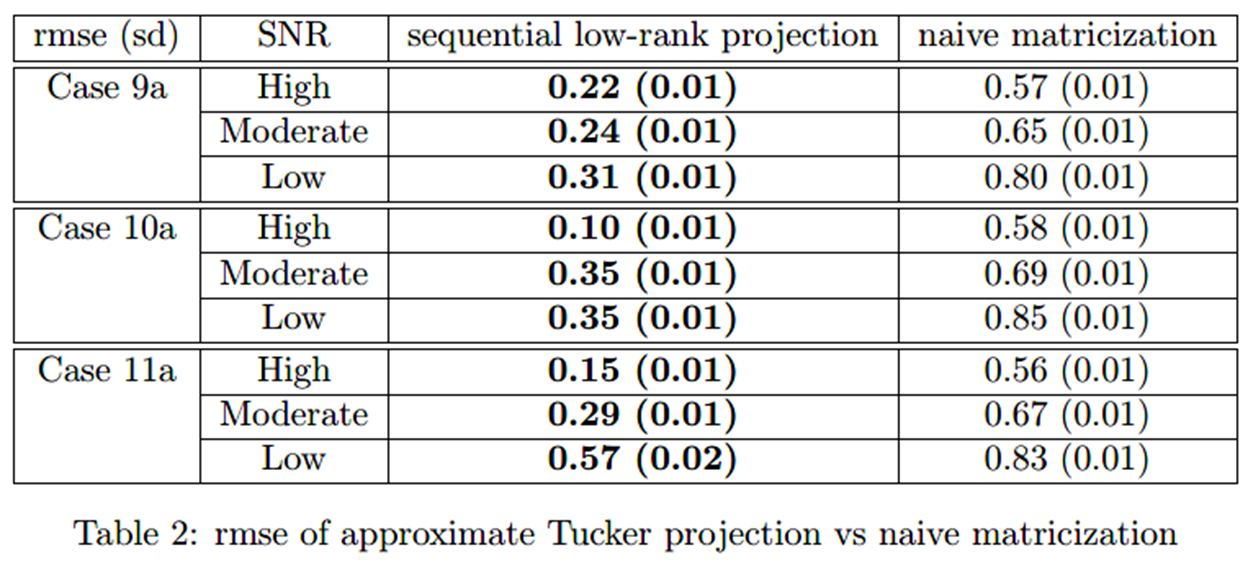
\includegraphics[width=.7\linewidth]{image039.png}
		\end{figure}
	\end{frame}
	
	
\end{document}